\subsection{Non-Embedding Based Comparison}
\label{sec:non_embedding_comparison}

In practice, the vocabulary sizes are different across different models, and embedding layers commonly account for relatively lower compute per parameter. We also note that the naming of different models has no consensus on using total parameters or non-embedding parameters in the model name. Hence, to conduct a more complete comparison, we also take statistics on both total parameters and non-embedding parameters of different open-weight and fully open-source models, and report the results in \Cref{tab:model_params_comparison}. In addition, taking non-embedding parameter as the X-axis, we report an additional comparison in \Cref{fig:performance_comparison_on_nonembedding}. We find that our model still excels the frontier of fully open-source models, and approaches close to leading open-weight models, like the Qwen series of a similar scale. Our advantage over other fully open-source models looks more prominent when taking account the non-embedding parameters.

\begin{figure}[htbp]
    \centering
    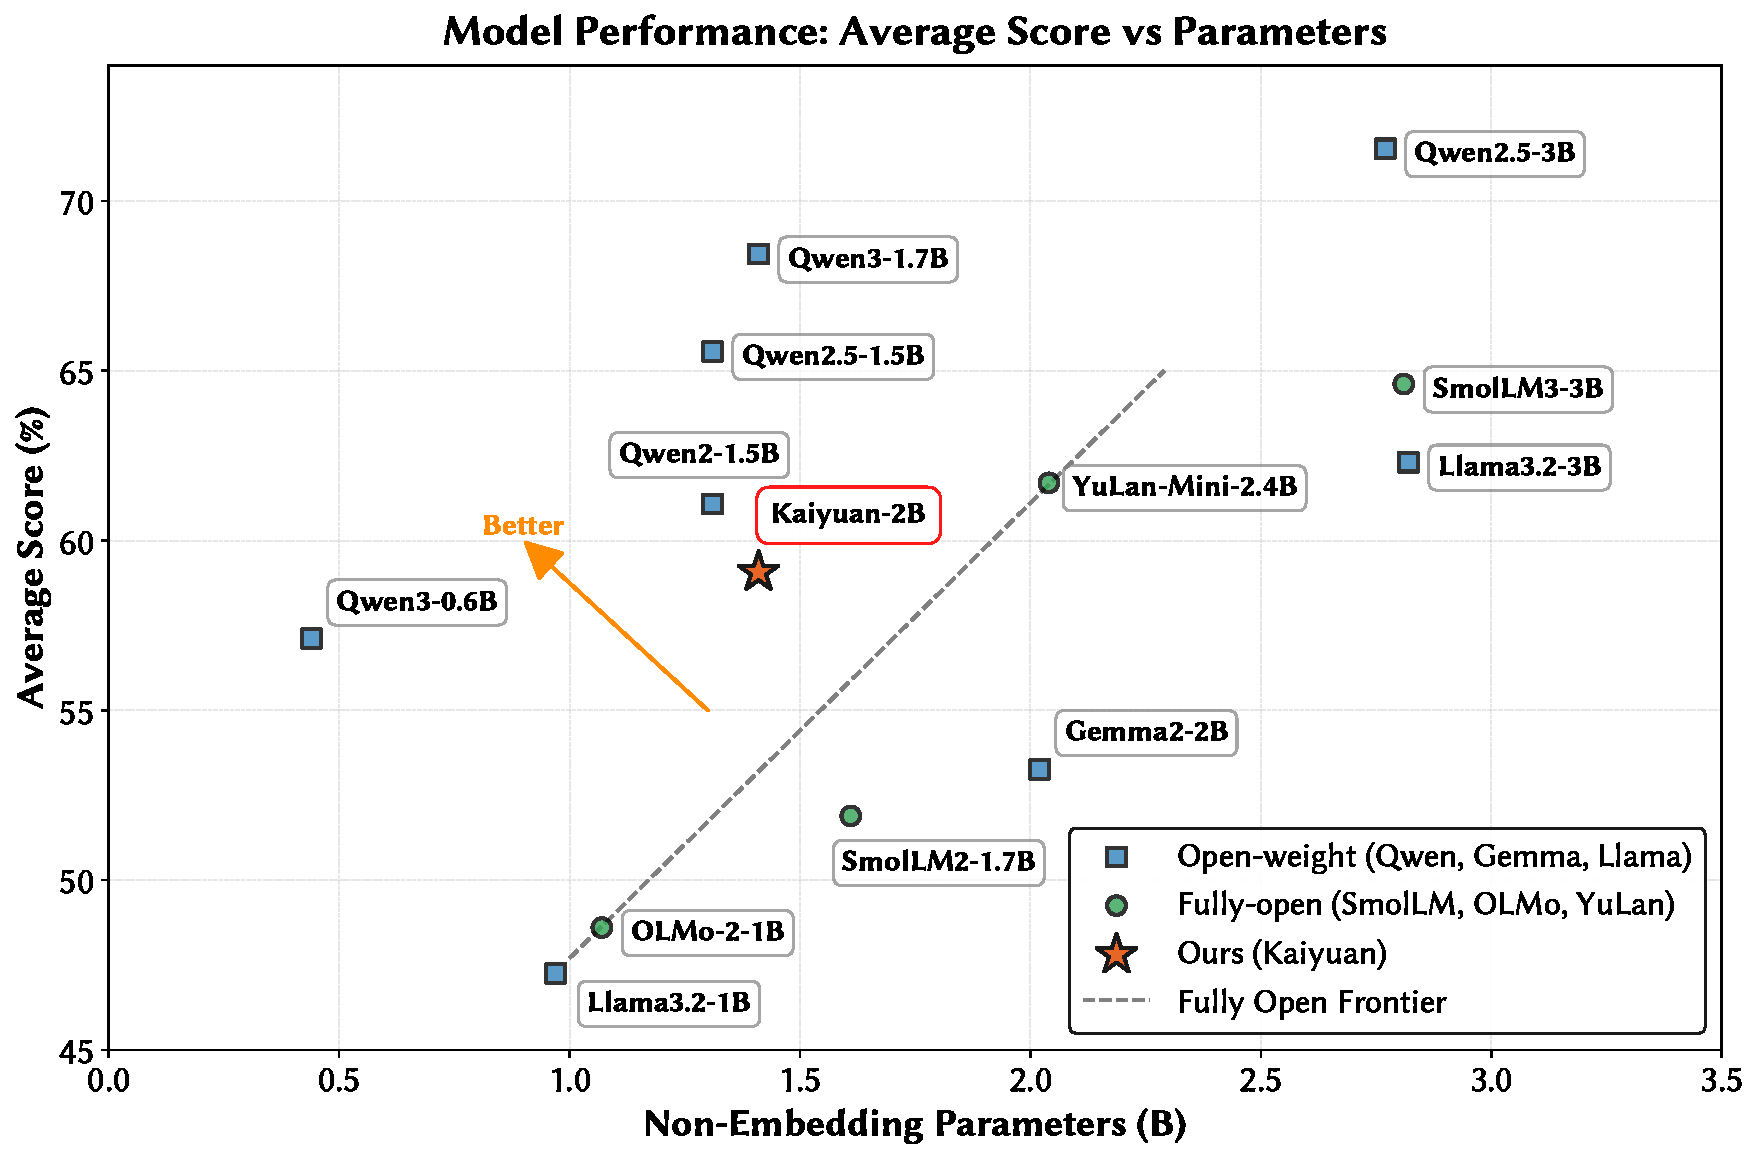
\includegraphics[width=\linewidth]{fig/model_performance_comparison_non_embedding.pdf}
    \caption{Model Performance Comparison over Non-embedding Parameters.}
    \label{fig:performance_comparison_on_nonembedding}
\end{figure}


\begin{table}[htbp]
\centering
\caption{Model Parameter Statistics Comparison.}
\label{tab:model_params_comparison}
\begin{tabular}{lcccc}
\toprule
\textbf{Model Name} & \textbf{Total} & \textbf{Embedding} & \textbf{Non-Embedding} & \textbf{Tied Embedding}\\
\midrule
\multicolumn{5}{l}{\textit{\textbf{SOTA Models}}} \\
\rowcolor{openweight} Qwen2-1.5B & 1.54B & 0.23B & 1.31B & TRUE\\
\rowcolor{openweight} Qwen2.5-1.5B & 1.54B & 0.23B & 1.31B & TRUE\\
\rowcolor{openweight} Qwen2.5-3B & 3.09B & 0.31B & 2.77B & TRUE\\
\rowcolor{openweight} Qwen3-0.6B-Base & 0.60B & 0.16B & 0.44B & TRUE\\
\rowcolor{openweight} Qwen3-1.7B-Base & 1.72B & 0.31B & 1.41B & TRUE\\
\rowcolor{openweight} Qwen3-4B-Base & 4.02B & 0.39B & 3.63B & TRUE\\
\rowcolor{openweight} Gemma-2-2B & 2.61B & 0.59B & 2.02B & TRUE\\
\rowcolor{openweight} Llama-3.2-1B & 1.24B & 0.26B & 0.97B & TRUE\\
\rowcolor{openweight} Llama-3.2-3B & 3.21B & 0.39B & 2.82B & TRUE\\
\multicolumn{5}{l}{\textit{\textbf{Fully-Open SOTA Models}}} \\
\rowcolor{fullyopen} SmolLM2-1.7B & 1.71B & 0.10B & 1.61B & TRUE\\
\rowcolor{fullyopen} OLMo-2-0425-1B & 1.48B & 0.41B & 1.07B & FALSE\\
\rowcolor{fullyopen} YuLan-Mini & 2.42B & 0.38B & 2.04B & FALSE\\
\rowcolor{fullyopen} SmolLM3-3B & 3.08B & 0.26B & 2.81B & TRUE\\
\multicolumn{5}{l}{\textit{\textbf{Ours}}} \\
\rowcolor{ours} PCMind-2.1-Kaiyuan-2B & 2.03B & 0.62B & 1.41B & FALSE\\
\bottomrule
\end{tabular}
\end{table}
